\chaptersub{Symmetric Modes}{Private Key Cryptography}

\section{Block Cipher Modes}\label{sec:blockciphermodes}
    A \textbf{block cipher} is type of encryption based on \textbf{permutation}, where they key, $\{0,1\}^k$, defines a transposition of bits in the block to the encrypted, $\{0,1\}^b$. The block is a proportion of the message.\\
    \\
    DES was the first civilian block cipher and was developed at IBM in the 1970s. When the US government adopted it, they recommended the following four ways to use it, these are now used with any block cipher.
    \begin{itemize}
        \item Electronic Code Book
        \item Cipher Block Chaining
        \item Counter
        \item ...
    \end{itemize}
    
    \subsection{Electronic Code Book}
    This is a very simple, it \textbf{divides} the message into blocks of size $b$, pads the last one, and \textbf{encrypts them all individually}, this is ineffective to say the least, as evidenced in Figure~\ref{fig:tux}. A block cipher using ECB is only OW-CPA, as Figure~\ref{fig:ecb-attacktable} says. 
    This is terrible!\\
    \begin{figure}[htp!]
    \centering
    \attacktable{owcpa}
    \caption{Security Models ECB passes}
    \label{fig:ecb-attacktable}
    \end{figure}
    \\
    The weakness of this mode lays in the fact that the blocks are encrypted independently. This is the basis for the two attacks below, but it also means it's susceptible to \textbf{block replay}. That is where an adversary edits a bit knowing how it will affect the decrypted message. If I knew you were sending me some money, and I knew the block containing the amount you were transferring, I could change that block in the hope I would end up with a larger transaction. This could be fixed with a checksum. ECB has one positive, an error in one block of the ciphertext will not propagate to other blocks during decryption.\\
    \\
    \textbf{Proving a cryptographic system passes a security model is beyond the scope of this course}, but you should be able to give an intuitive reason. It passes OW-CPA because, with only an encryption oracle, you would have to brute-force every possible message to match it with the ciphertext. We can always make $b$ large enough so that this is not possible\footnote{This might be possible if you knew the context of the message, if you understand what is being sent and the domain of possible values of a block is relatively small. This is simply poor implementation of the encryption, however, and we don't worry about that.}. Note that all the proofs for block cipher modes assume we are using a `perfect block cipher'.\\
    \\
    \textbf{OW-CCA Example:} We can win a OW-CCA game by kind of cheating in the following way. If we have a decryption oracle, we can decrypt anything that is not the message. Since the blocks are independent, we can simply split the message in half and decrypt both individually and then concatenate the result.\\
    \\
    \textbf{IND-PASS Example:} In an indistinguishability game we decide the two messages sent to the oracle (of which one will be encrypted). Again we use the fact that the blocks are encrypted independently, and give one of the messages as a bit string concatenated onto itself, $m_0=b_1||b_1$. If the ciphertext can be split into two equal bit strings in the same way, then $m_0$ was encrypted, else $m_1$.
    
    \subsection{Cipher Block Chaining}
    Cipher Block Chaining removes a lot of the problems found in ECB by XORing each block with the previously encrypted block --- incorporating a dependence on the previous block. The first block of the ciphertext is called the \textbf{Initalisation Vector} (IV), and is what the first block of the message is XOR-ed with.\\
    \begin{figure}[htp!]
        \centering
        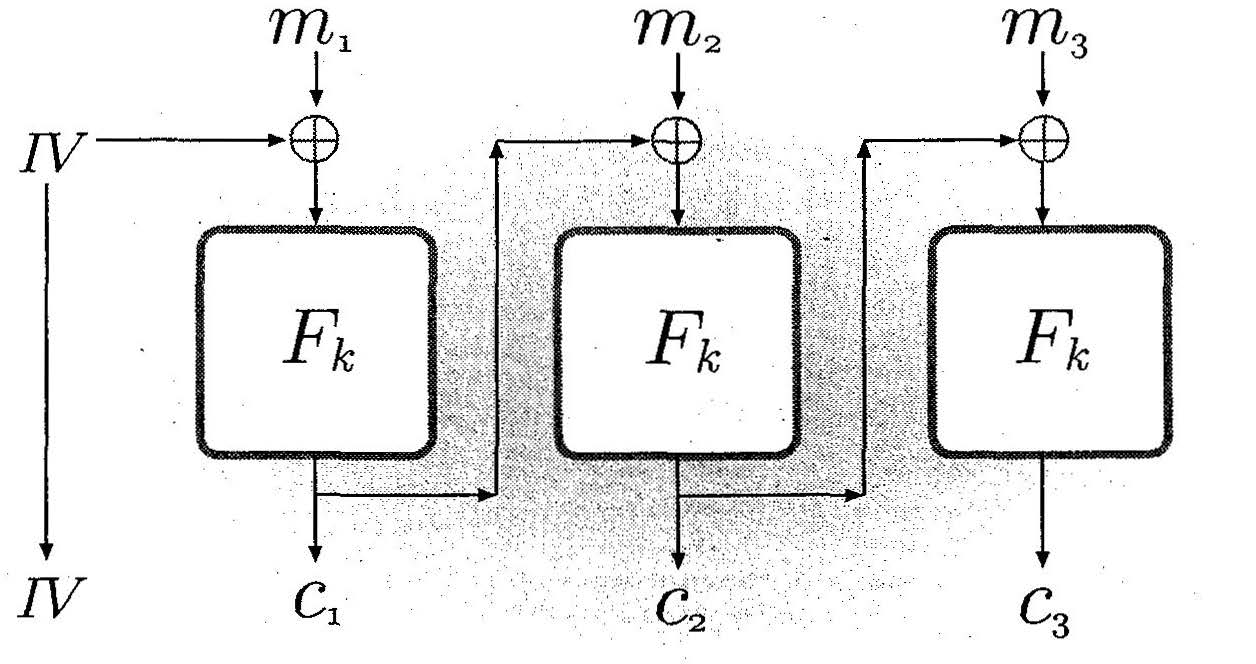
\includegraphics[width=10cm]{img/cbc}
        \caption{Diagram of CBC encrypting}
    \end{figure}
    \\
    More formally:\nopagebreak
    \begin{center}
    \begin{tabular}{lll}
    \textbf{Encryption}:                                        && \textbf{Decryption}\\
    $\csubc{0} = IV$                                                  && $IV = \csubc{0}$\\
    $\csubc{1} = Enc_\ck(\csubm{1} \oplus IV)$                                && $\csubm{1} = Dec_\ck(c_1) \oplus IV$\\
    $\csubc{i} = Enc_\ck(\csubm{i} \oplus \csubc{i-1}) \textrm{ for } i > 1$      && $\csubm{i} = Dec_\ck(c_i) \oplus \csubc{i-1} \textrm{ for } i > 1$\\
    \end{tabular}
    \end{center}
    \begin{figure}[htp!]
        \centering
        \attacktable{indcpa}
        \caption{Security of Models CBC}
        \label{fig:cbc-attacktable}
    \end{figure}
    Note that $IV$ is sent unencrypted, because it is needed for decryption. This can seem pointless, but if it is generated randomly every time, then it means that encryption is probabilistic. CBC is OW-CPA and IND-CPA but not OW-CCA or IND-CCA.\\
    \begin{figure}[htp!]
        \centering
        \begin{subfigure}[b]{0.3\textwidth}
            \centering
            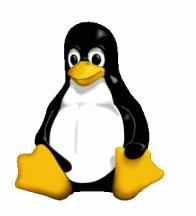
\includegraphics[width=\textwidth]{img/Tux.jpg}
            \caption{Original Image}
        \end{subfigure}
        \begin{subfigure}[b]{0.3\textwidth}
            \centering
            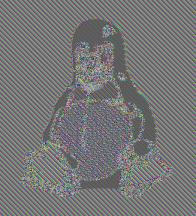
\includegraphics[width=\textwidth]{img/Tux_ecb.jpg}
            \caption{Encrypted using ECB}
        \end{subfigure}
        \begin{subfigure}[b]{0.3\textwidth}
            \centering
            
\includegraphics[width=\textwidth]{img/Tux_secure.jpg}
            \caption{Encrypted using CBC}
        \end{subfigure}
        \caption{Bitmap image of Tux being encrypted using ECB and CBC.}
        \label{fig:tux}
    \end{figure}
    \\
    \textbf{With a decryption oracle, CBC will fail} because of the same trick used before --- we can ask to oracle to decrypt the ciphertext with extra blocks on the end.
    
    
    
    \subsection{Counter Mode}
    Counter mode basically uses a stream cipher to generate a pseudo-random bit-string which can be one-time-padded with message. As Figure~\ref{fig:ctr} shows, the algorithm generates a $IV$ ($IV \leftarrow \{0,1\}^n$) and increments this by one for every block. The $IV+n$ values are then put through the block cipher to generate the bit-string. In all the material, the $IV$ is refereed to as $ctr$ for this algorithm.\\
    \begin{figure}[htp!]
        \centering
        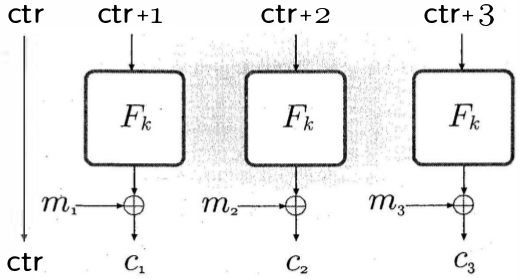
\includegraphics[width=0.5\textwidth]{img/ctr.png}
        \caption{Diagram of CTR mode}
        \label{fig:ctr}
    \end{figure}
    \\
    Formally:
    \begin{center}
        \begin{tabular}{lll}
            \textbf{Encryption:} && \textbf{Decryption:}\\
            $\csubc{0} = IV$ && $IV = \csubc{0}$\\
            $\csubc{i} = Enc_\ck(IV + i) \oplus \csubm{i}$ && $m_i = Enc_\ck(IV + i) \oplus \csubc{i}$
        \end{tabular}
    \end{center}
    CTR mode passes the same security modes as CBC (Figure~\ref{fig:ctr-attacktable}). But it has one positive over CBC: decrypting a block is not dependent on the decryption of the previous block, meaning that we can parallelise decryption (and encryption for that matter).
    \begin{figure}[htp!]
        \centering
        \attacktable{indcpa}
        \caption{Security of Models CTR}
        \label{fig:ctr-attacktable}
    \end{figure}





\section{S-Box \& Analysis}\label{sec:sbox}
    Until now, we haven't talked about what happens in the $Enc$ function. In there, there is a mixture of \textbf{substition} of characters for other characters\footnote{Think of Caesar's cipher where a letter is moved $n$ places in the alphabet, where $n$ is defined in the key} and \textbf{permutations}, where bits (or larger groupings of bits) change position. When there is this mixture of subtition and permutation, we give it the imaginative name of a `substitution-permutation network'.\\
    \\
    One method an attacker might use is called a \textbf{known-plaintext attack}, where they have the \textit{plaintext} and \textit{ciphertext} and try to work the key out from these. This means we need a large number of keys, so that an exhaustive keysearch is not possible. We also have to make sure that the block size is large enough, since we could store known block decryptions and decipher a large part of the ciphertext through this (\textbf{text dictionary attack}).\\
    \begin{table}[htp!]
        \centering
        \begin{tabular}{lccccccccccccccccccccccccccc}
            \toprule
            Input & 0 & 1 & 2 & 3 & 4 & 5 & 6 & 7 & 8 & 9 & A & B & C & D  & E & F\\
            \midrule
            Output & E & 4 & D & 1 & 2 & F & B & 8 & 3 & A & 6 & C & 5 & 9 & E & 7\\
            \bottomrule
        \end{tabular}
        \caption{Example of a look-up table for an S-Box}
        \label{fig:lookupsbox}
    \end{table}
    \\
    An \textbf{S-Box} is a mapping of bit-strings to other bit-strings, theses do not have to be the same length, but if they are not, the output is almost always of a shorter length. Table~\ref{fig:lookupsbox} shows an example of an S-Box which maps 4-bit strings to 4-bit strings. We want to make the substitution as \textbf{non-linear} as possible. Formally, it would be linear if Equation~\ref{equ:sboxlin} was true, or at least was true was large probability.
    % FIXME: Line above ends in confusing way.
    
    \subsection{Differential Analysis}
    At the heart of a number of the techniques used to successfully beat crypto games in Section~\ref{sec:blockciphermodes}, was that we get around the constraint of not being allowed to send the message or ciphertext to an oracle by changing it into something we know will still give us something useful. With a linear S-Box, we (as an attacker) would be able to transform the message/ciphertext and then perform another transformation on the oracles response.
    \begin{equation}
        \begin{array}{l}
            \csubm{1} \rightarrow \csubc{1}\\
            \csubm{2} \rightarrow \csubc{2}
        \end{array}\Bigr\}
        \Rightarrow
        (\csubm{1} + \csubm{2}) \rightarrow (\csubc{1} + \csubc{2})
        \label{equ:sboxlin}
    \end{equation}
    To find patterns that we can exploit to do this, we perform \textbf{differential analysis} on the S-Box. Differential analysis \textit{tabulate[s] specific differences in the input that lead to specific differences in the output with probability greater than would be expected for a random permutation}. This would tell us whether adding 5 to the input will always give us an output 10 too large.\\
    \\
    To do this, we make a table with all the inputs against all the outputs. Then we take \textbf{every pair of inputs}, $(s_1,s_2)$, calculate there difference, $\Delta s=s_1\oplus s_2$, and the the difference between the outputs of those inputs, $\Delta t = \mathbb{S}(s_1) \oplus \mathbb{S}(s_2)$. Figure~\ref{fig:diffanalpair} gives an example of this. For each pair, we add one to the value at $(\Delta s,\Delta t)$, so that cell $(s,t)$ gives us the number of times a difference of $s$ in the input caused a difference in $t$ in the output.
    \begin{figure}[htp!]
        \begin{align*}
            s_1=3=0011_2   && t_1=\mathbb{S}(s_1) = 1 &= 0001_2  &&  \Delta s=s_1\oplus s_2=5=0101_2\\
            s_2=6=0110_2   && t_2=\mathbb{S}(s_2) = B &= 1011_2  &&  \Delta t=t_1\oplus t_2=A=1010_2
        \end{align*}
        \caption{Example of differential analysis for the pair of inputs $(3,6)$}
        \label{fig:diffanalpair}
    \end{figure}
    \\
    Although its unlikely that the table will show all differences in the input of $s$ lead to an output difference of $t$, even a \textit{better than chance} difference gives a cryptanalyst a much smaller space for them them brute force. A perfect S-Box would have a 1 in every cell, but this is \textit{impossible}. We can measure an S-Boxes quality by how close to a \textbf{uniform distribution} it has in this table.
    \subsection{Linear Analysis}
        Linear analysis consists of two parts. The first is to \textbf{construct linear equations} describing relationships between the \textit{plaintext}, \textit{ciphertext} and \textit{key bits} that have a high bias; that is, whose probability of being true is close to 0 or 1.  The second is to use these linear equations in conjunction with known plaintext-ciphertext pairs to derive key bits.\\
        \\
        The notes write a linear equation for an S-Box has n input bits $X_i$ and m-output bits $Y_i$, as

        \begin{equation}
            L_{I,J} = (X_{i_1} \oplus \cdots \oplus X_{i_2}) \oplus (Y_{i_1} \oplus \cdots \oplus Y_{i_2})
        \end{equation}
        \begin{align*}
            \text{where, } & I = \{i_1, \cdots ,i_u\} \subset \{1, \cdots ,n\}\\
            & J = \{j_1, \cdots ,j_u\} \subset \{1, \cdots ,n\}
        \end{align*}
        because they apparently don't want you to understand it. It just means that $L$ is a function taking bits from specific positions from the input and output and XORing them all. Eg, $L_1 = X_1 \oplus X_3 \oplus X_4 \oplus Y_2$.\\
        \\
        For each linear equation, $L_i$, we calculate the probability that for a random input, $X$, the function will return 0: $p=Pr[L_i=0]$. To obtain the bias, we just subtract $-0.5$ from this probability, making the bias in a range of -0.5 to 0.5.\\
        \\
        If function has a large enough bias (either positive or negative), then we can approximate the whole cipher as a linear function. Using this method we can prove that an S-Box is non-linear.

\section{AES --- Rijndael}
    Some ciphers involve repeating a weaker `round function' to make a stronger encryption. Round functions will output bit-strings the same size of the input, and they must be a revertible one-to-one function, so that we can decrypt the ciphertext. The notation usually uses $r$ for the number of rounds, $n$ for the block size and $s$ for the key size. Each round uses a different key, and these sub-keys are all derived from the main key. A block is usually represented as a matrix holding all the bytes. Each state of the encryption is applied to the `state matrix', $s$.\\
    \\
    ASE is an encryption scheme which uses round functions. Its works on 128-bit blocks, uses keys of 128/192/256-bits and works on 10/12/14. Each round consists of the following operations:\\
    \\
    \newcommand{\leftminipagewidth}{0.3\textwidth}
    \newcommand{\rightminipagewidth}{0.7\textwidth}
    \begin{tabular}{ll}
        \begin{minipage}[t]{\leftminipagewidth}
            \textbf{Byte Substitution}\\
            Just apply the S-Box to the block.
        \end{minipage}
        &
        \begin{minipage}[t]{\rightminipagewidth}
        $
            \begin{pmatrix}
                s_{0,0} & s_{0,1} & s_{0,2}\\
                s_{1,0} & s_{1,1} & s_{1,2}\\
                s_{2,0} & s_{2,1} & s_{2,2}
            \end{pmatrix}
            \rightarrow
            \begin{pmatrix}
                \mathbb{S}(s_{0,0}) & \mathbb{S}(s_{0,1}) & \mathbb{S}(s_{0,2})\\
                \mathbb{S}(s_{1,0}) & \mathbb{S}(s_{1,1}) & \mathbb{S}(s_{1,2})\\
                \mathbb{S}(s_{2,0}) & \mathbb{S}(s_{2,1}) & \mathbb{S}(s_{2,2})
            \end{pmatrix}
        $
        \end{minipage}

        \\\\

        \begin{minipage}[t]{\leftminipagewidth}
            \textbf{Shift Rows}
            Shift a row, so that message is diffused over the columns.
        \end{minipage}
        &
        \begin{minipage}[t]{\rightminipagewidth}
        $
            \begin{pmatrix}
                \textcolor{red}{s_{0,0}} & \textcolor{green}{s_{0,1}} & \textcolor{blue}{s_{0,2}}\\
                \textcolor{red}{s_{1,0}} & \textcolor{green}{s_{1,1}} & \textcolor{blue}{s_{1,2}}\\
                \textcolor{red}{s_{2,0}} & \textcolor{green}{s_{2,1}} & \textcolor{blue}{s_{2,2}}
            \end{pmatrix}
            \rightarrow
            \begin{pmatrix}
                \textcolor{red}{s_{0,0}} & \textcolor{green}{s_{0,1}} & \textcolor{blue}{s_{0,2}}\\
                \textcolor{green}{s_{1,1}} & \textcolor{blue}{s_{1,2}} & \textcolor{red}{s_{1,0}}\\
                \textcolor{red}{s_{2,0}} & \textcolor{green}{s_{2,1}} & \textcolor{blue}{s_{2,2}}
            \end{pmatrix}
        $
        \end{minipage}

        \\\\

        \begin{minipage}[t]{\leftminipagewidth}
            \textbf{Mix Column}\\
            Can choose a matrix to multiply by. Diffuses over rows. \footnotemark
        \end{minipage}
        &
        \begin{minipage}[t]{\rightminipagewidth}
        $
            \begin{pmatrix}
                s_{0,0} & s_{0,1} & s_{0,2}\\
                s_{1,0} & s_{1,1} & s_{1,2}\\
                s_{2,0} & s_{2,1} & s_{2,2}
            \end{pmatrix}
            \rightarrow
            \begin{pmatrix}
                2 & 3 & 1\\
                1 & 1 & 4\\
                3 & 1 & 1
            \end{pmatrix}
            \begin{pmatrix}
                s_{0,0} & s_{0,1} & s_{0,2}\\
                s_{1,0} & s_{1,1} & s_{1,2}\\
                s_{2,0} & s_{2,1} & s_{2,2}
            \end{pmatrix}
        $
        \end{minipage}

        \\\\

        \begin{minipage}[t]{\leftminipagewidth}
            \textbf{Round Key Addition}\\
            XOR with the round key.
        \end{minipage}
        &
        \begin{minipage}[t]{\rightminipagewidth}
        $
            \begin{pmatrix}
                s_{0,0} & s_{0,1} & s_{0,2}\\
                s_{1,0} & s_{1,1} & s_{1,2}\\
                s_{2,0} & s_{2,1} & s_{2,2}
            \end{pmatrix}
            \rightarrow
            \begin{pmatrix}
                k_{0,0} & k_{0,1} & k_{0,2}\\
                k_{1,0} & k_{1,1} & k_{1,2}\\
                k_{2,0} & k_{2,1} & k_{2,2}
            \end{pmatrix}
            \oplus
            \begin{pmatrix}
                s_{0,0} & s_{0,1} & s_{0,2}\\
                s_{1,0} & s_{1,1} & s_{1,2}\\
                s_{2,0} & s_{2,1} & s_{2,2}
            \end{pmatrix}
        $
        \end{minipage}

    \end{tabular}\\\\
    \footnotetext{The aim is to defuse the message as much as possible, so a maximal distance algorithm is used to find the matrix which will do this the most --- you don't need to worry about that though.}
    It's possible that you need to know they are put together in AES, so you can see the pseudo-code in Algorithm~\ref{alg:aes}. Basically, every round the sub-key is added, then the S-Box is applied, then the rows are shifted, then the columns are mixed. In the last round the columns aren't mixed though.\\
    \begin{figure}[htp!]
        \centering
        \begin{algorithm}[H]
            \SetAlgoLined
            AddRoundKey($S$,$K_0$]);\\
            \For{$i\leftarrow 1$ \KwTo $9$}{
                SubBytes($S$);\\
                ShiftRows($S$);\\
                MixColumns($S$);\\
                AddRoundKey($S$,$K_i$);\\
            }
            SubBytes($S$);\\
            ShiftRows($S$);\\
            \caption{AES}
            \label{alg:aes}
        \end{algorithm}
    \end{figure}
    \\
    \textbf{Write section on Key Scheduling}\\
    \\
    In Section~\ref{sec:sbox}, we loo

\section{Message Authentication}
    \subsection{Why Do This}
        Encrypting data provides confidentiality (remember the three goals), but does not provide authenticity or integrity without additional sauce. This is the additional sauce.
        It comes with two flavours that are used for different things: \textbf{MDC} (Manipulation Detection Codes) and \textbf{MAC} (Message Authentication Codes). We will mainly worry about \textbf{MAC} stuff.
        The reason we use these at all is that they are the secret ingredient in getting from IND-CPA to the mythical, coveted IND-CCA level of security.


    \subsection{\textbf{M}essage \textbf{A}uthentication \textbf{C}odes, you say?}
    MAC codes are the result of hashing the message, using a hash function that takes a key.
    \begin{figure}[htp!]
        \centering
        MAC = $h_{\ck}(\cm)$
    \end{figure}
    You would then typically send the MAC concatenated at the end of the message. The hash function, as per Kerckhoff's principle, is publicly described. Given $\ck$ and $\cm$, computing $h_{\ck}(\cm)$ should be easy.
    Given only $\cm$, computing a correct hash should be very difficult, even if several message-to-hash pairs are already known.\\
    \\
    A hash function is simply a surjective mapping from arbitrarily long strings to fixed length hash strings.

    \subsection{Security Model}
    Our security models are simple:
    \begin{itemize}
        \item \textbf{EF-PASS}: The passive attack where the bad guy can generate a valid MAC for any message, gibberish or otherwise. 
        \textbf{Existential} forgery is where the message may just be random rubbish, \textbf{Selective} forgery is creating a MAC for a specific message.

        \item \textbf{EF-CMA}: As above, but the douche of an adversary has an oracle that can perform MAC generation on other messages of his choice (but not the target message). This is the \textbf{Chosen Message Attack}
    \end{itemize}
    We will now look at two games for Existential Forgery; as a MAC may be probabilistic, we define two algorithms for these games:

    \begin{itemize}
        \item $\textbf{MAC}_{\ck}(\cm)$: Generates the MAC for message \emph{\cm}.
        \item $V_{\ck}(\cm, \cc)$: A boolean-returning verification function. True is good. False is bad. Get with the program, kids. Also this may not simply be a case of recomputing the MAC; if the algorithm that generates it is probabilistic, we need other methods of checking correctness.
    \end{itemize}
    It is a given that our opponent has access to a Verification Oracle (otherwise how will they know if they have cracked it?). 

    \begin{figure}[htp!]
    \centering
    \begin{subfigure}[b]{0.4\textwidth}
        \centering
        \begin{cryptogame}{}
            \cgameright{$V(\cm, \cc)$}
            \cgameleft{$\cmast$, $\ccast$}
        \end{cryptogame}
        \caption{EF-PASS: Passive Attack}
        \label{fig:ef-pass}
    \end{subfigure}
    ~
    \begin{subfigure}[b]{0.4\textwidth}
        \centering
        \begin{cryptogame}{}
            \cgameright{$V(\cm, \cc)$}
            \cgameright{$c = MAC_{\ck}(\cm)$}
            \cgameleft{$\cmast$, $\ccast$}
        \end{cryptogame}
        \caption{EF-CMA: Chosen Message Attack}
        \label{fig:ef-cma}
    \end{subfigure}
    \caption{MAC security games}
    \label{fig:ef-games}
\end{figure}

    There exists a `Strong Forgery' variant of \textbf{EF-CMA} called, unsuprisingly, \textbf{SF-CMA}, which changes the restriction on the MAC oracle to be that whilst $m^{*}$ can be passed to the oracle, $c^{*}$ must not have been returned.

    Assuming we can create a MAC function that achieves this, we can now make INC-CCA symmetric encryption schemes! Hooray!

    There exists a `Strong Forgery' variant of \textbf{EF-CMA} called, unsuprisingly, \textbf{SF-CMA}, which changes the restriction on the MAC oracle to be that whilst $\cmast$ can be passed to the oracle, $\ccast$ must not have been returned.\\
    \\
    Assuming we can create a MAC function that achieves this, we can now make INC-CCA symmetric encryption schemes! Hooray!

    \subsection{IND-CCA Here We Come}
    The reason that CBC and CTR modes, whilst groovy, were not \textbf{IND-CCA} was that an attacker could look at our ciphertext and construct a related one which could be decrypted through their oracle, giving them a related plaintext.

    MAC prevents them from doing that! Sweet! So to make an \textbf{IND-CCA} secure scheme you will need:
    \begin{itemize}
        \item One \textbf{IND-CPA} secure symmetric cipher \emph{E}.
        \item One \emph{SECURE}\footnote{i.e. Cannot produce a valid \textbf{MAC} without access to the correct key} \textbf{MAC} function \emph{MAC}.
        \item One hybrid key consisting of $\csubk{0}$ and $\csubk{1}$ which are the keys for \emph{E} and \emph{MAC} respectively.
    \end{itemize}

    We can then construct encryption and decryption thusly:
    \begin{figure}[htp!]
    \centering
    \raisebox{-0.5\height}{
        \begin{subfigure}[b]{0.4\textwidth}
            \centering
            \textbf{Encrypt}
            \begin{enumerate}
                \item Split $\ck$ into $\csubk{0}$ and $\csubk{1}$
                \item $\csubc{0} = E_{\csubk{0}}(\cm)$
                \item $\csubc{1} = MAC_{\csubk{1}}(\csubc{0})$
                \item And voila: $\cc = (\csubc{0}, \csubc{1})$
            \end{enumerate}
            \label{fig:ind-cca-enc}
        \end{subfigure}
        }
    ~
    \raisebox{-0.5\height}{
        \begin{subfigure}[b]{0.4\textwidth}
            \centering
            \textbf{Decrypt}
            \begin{enumerate}
                \item Split $\ck$ into $\csubk{0}$ and $\csubk{1}$
                \item Split $\cc$ into $\csubc{0}$ and $\csubc{1}$
                \item $\csubcast{1} = MAC_{\csubk{1}}(\csubc{0})$
                \item If $\csubcast{1} \neq \csubc{1}$ then ABORT and return $\bot$
                \item Else return $\cm$ where $\cm = D_{\csubk{0}}(\csubc{0})$ 
            \end{enumerate}
            \label{fig:ind-cca-dec}
        \end{subfigure}
    }
    \caption{How To Make an IND-CCA Scheme}
    \label{fig:ind-cca-ed}
    \end{figure}

    This obviously involves the ciphertext being expanded (more than it might be already) because it includes a MAC. 

    With the MAC allowing us to validate a ciphertext as being `authentic', this type of scheme is often called \emph{`authenticated encryption'}.
    It is important to realise the \textbf{very important} distinction between this idea, which is that a ciphertext is authentic, and the concept that a ciphertext came from where it was supposed to, which is part of the regular cryptographic definition of `Authenticity'.

    \subsection{How To Make A MAC}
    There are a few types of MAC schemes, from MACs that are custom made for that specific encryption scheme to MACs that are derived from MDCs (Manipulation Detection Codes).

    The most popular, and exceedingly examinable, variants that we look at are all based on CBC-mode block ciphers. They are covered by various international standards\footnote{Gotta love standards. Thrilling stuff} and are very widely used. We shall refer to schemes like this under the title of CBC-MAC. Like this...

    \subsection{CBC-MAC}
    CBC-MAC is pretty much a straightforward application of a block cipher (like DES or AES). We just have to add the MAC on after padding the ciphertext.\\
    \\
    Given our cipher, which operates on blocks of \emph{b} bits, we can make a MAC really simply; assuming we have \emph{q} data blocks in our message, $\csubm{1}, \csubm{2}...m_{q}$, we would do as follows:

    \begin{enumerate}
        \item Set initial intermediate variables: $I_{1} = \csubm{1}, O_{1} = e_{\ck}(I_{1})$
        \item For $i = 2, 3 ... q$:
            \begin{itemize}
                \item $I_{i} = \csubm{i} \oplus O_{i - 1}$
                \item $O_{i} = e_{\ck}(I_{i})$
            \end{itemize}
        \item Do any post-processing you want on $O_{q}$.
        \item Truncate if necessary to $m$ bits and serve piping hot.
    \end{enumerate}
    In terms of padding the ciphertext, there are 3 schemes suggested in those groovy groovy standards. All of these pad to a whole number of blocks.
    \begin{itemize}
        \item Just add zeroes. Easy, right?
        \item Add a single 1, then trail out with zeroes.
        \item Pad with zeroes until you get a whole number of blocks, then add a block containing the length of the unpadded message.
    \end{itemize}
    In terms of optional post-processing, there are two specified methods:
    \begin{itemize}
        \item Choose another key, $\csubk{1}$, and replace $O_{q}$ with $e_{\ck}(d_{\csubk{1}}(O_{q}))$
        \item Choose another key, $\csubk{1}$, and replace $O_{q}$ with $e_{\ck_{1}}(O_{\cq})$ 
    \end{itemize}
    Either one of those can make it much harder to do a brute force search for $k$. Which is a good thing, young padawan. Oh yes.

    \subsection{Hashing}
    Like we said, hashing in this case is just an efficient function mapping arbritrarily long binary strings to fixed length binary strings. Simples.\\
    \\
    Incidentally, these hashes are essentially MCDs, though they are not called that now. Used to be the case that you'd do a hash (MDC), concatenate it to the message and then encrypt that. The problem with a concatenate-then-encrypt scheme under CBC is that an attacker can create a message that consists of the message they wish to send, a hash for it, and then some other random guff, and then hash that (this is a CPA method). If the attack then truncates the resulting ciphertext they get their valid target ciphertext, complete with hash.\\
    % TODO: EXPLAIN THIS BETTER DRUMMOND YOU CRAZY MAN.
    \\
    While earlier we talked about hashing with a key, in practice hash functions don't have a key. It is often simpler to consider a family of functions, and require three conditions of them:
    \begin{enumerate}
        \item Preimage Resistance: given $\cc = h(\cm)$, hard to find another $\cm^{'}$ such that $h(\cm^{'}) = \cc = h(\cm)$
        \item 2nd Preimage Resistance: The same as preimage resistance, except that we are also given $\cm$.
        \item Collision Resistance: hard to find $\cm, \cm^{'} \neq \cm$ such that $h(\cm) = h(\cm^{'})$
    \end{enumerate}
    Typical practical choices for a cryptographic hash are the SHA family, or the RIPEMD family. % What the fuck is a RIPEMD? Sounds bad lol. - Matt

    \subsection{From Hash To MAC}

    Given a hash function, how can we bung a key in there sensibly? There are the simple prefix, suffix and envelope methods, though these are not secure.
    \begin{itemize}
        \item With prefixing it is possible to calculate $MAC_{\ck}(\cm||\cm^{'})$ without knowing the key. Simply split your intended message in half, and you're good to go. Exact method not shown in notes.
        \item Suffixing suffers from a weakness that makes it easier to find collisions in the hash function; this can be done offline, as well, so you do not need to send lots of queries to the target. Exact methodology not disclosed in notes.
        \item Envelope method with padding: The reason this isn't secure isn't given in the notes, and I can't find it online. % TODO: SOMEONE HELP ME OH GOD PLEASE
    \end{itemize}
    It is better to use HMAC (keyed-\textbf{H}ash \textbf{M}essage \textbf{A}uthentication \textbf{C}ode):
    $$HMAC_{\ck}(\cm) = h(\ck||p_{1}||h(\ck||p_{2}||\cm))$$
    Where $p_{1}$ and $p_{2}$ are fixed strings used to pad $\ck$ to a full block.\\
    \\
    You can use both MDC and MAC for data integrity, with or without confidentiality.\\
    \\
    Without confidentiality:
    \begin{itemize}
        \item \textbf{MAC}: compute $MAC_{\ck}(\cm)$ and send $\cm||MAC_{\ck}(\cm)$
        \item \textbf{MDC}: Send $h(\cm)$ over a seperate, authenticated channel.
    \end{itemize}
    With confidentiality:
    \begin{itemize}
        \item \textbf{MAC}: need two different keys, $k_{1}$ and $k_{2}$
        \begin{itemize}
            \item $\csubk{1}$ is for computing $\cc = e_{\csubk{1}}(\cm)$
            \item $\csubk{2}$ if for computing $MAC_{\csubk{2}}(\cc)$, which you append to $\cc$ before sending that combined string.
        \end{itemize}
        \item \textbf{MDC}: we only need one key $k$ for encryption, where we send $\cc = e_{\ck}(\cm||h(\cm))$, but as we discussed earlier this can be compromised by a man in the middle attack.
    \end{itemize}
